\documentclass[12pt,a4paper]{article}
\usepackage[utf8]{inputenc}
\usepackage[slovak]{babel}
\usepackage[T1]{fontenc}
\usepackage[a4paper, margin=2.5cm]{geometry}
\usepackage{fancyhdr}
\usepackage{titlesec}
\usepackage{enumitem}
\usepackage[hidelinks]{hyperref}
\usepackage{tikz}
\usetikzlibrary{arrows.meta, positioning}
\usepackage{bytefield}
\usepackage{graphicx}
\usepackage{subcaption}
\usepackage{rotating}
\usepackage[table,xcdraw]{xcolor}
\usepackage{longtable}
\usepackage{booktabs}
\usepackage{xcolor}
\usepackage{enumerate}
\usepackage{soul}
\usepackage{etoolbox}
\robustify\hl

\definecolor{highlight}{rgb}{0.56, 0.74, 0.56}
\definecolor{shade}{rgb}{0.8, 0.8, 0.8}
\definecolor{notmentioned}{rgb}{1, 0.74, 0.78}


\sethlcolor{notmentioned}

% Header setup
\pagestyle{fancy}
\fancyhf{}
\fancyhead[L]{\textbf{Počítačová bezpečnosť – \leftmark}}
\fancyfoot[C]{\thepage}

% Section formatting
\titleformat{\section}{\Large\bfseries}{\thesection.}{1em}{}
\titlespacing*{\section}{0pt}{0pt}{1em}

\setlist[itemize]{noitemsep, topsep=0.2em, left=1.5em}

\begin{document}

\tableofcontents
\newpage

\newcommand{\examquestion}[2]{
    \clearpage
    \section{#1}
    \markboth{#1}{#1}
        #2
}

% ---- QUESTIONS ----




\examquestion{Riadenie prístupu v OS a aplikáciách}{
    \subsection{Motivácia, ciele, hrozby, príklady zraniteľností}
    \subsection{Používatelia a skupiny používateľov}
    \begin{itemize}
        \item Poznáme subjekty a objekty.
        \begin{itemize}
            \item Subjekt -- aktívna entita (osoba, zariadenie, proces), spôsobuje zmenu stavu systému alebo tok informácií medzi objektmi.
            \item Objekt -- pasívna entita súvisiaca s informačným systémom (zariadenie, súbor, proces, program, tabuľka a pod.), obsahuje alebo prijíma informácie.
            \begin{itemize}
                \item Prístup subjektu k objektu -- subjekt pristupuje k informáciám v objekte.
            \end{itemize}
        \end{itemize}
        \item Riadenie prístupu -- proces udeľovania alebo zamietania konkrétnych žiadostí o:
        \begin{itemize}
            \item získanie a používanie informácií a súvisiacich služieb spracovania informácií
            \item vstup do konkrétnych fyzických zariadení (napr. federálne budovy, vojenské zariadenia, vstupy na hraničné priechody)
        \end{itemize}
    \end{itemize}
    \subsection{Riadenie prístupu v OS: modely, MAC, DAC, RBAC, ACL, prístupové práva, SELinux a pod.}
    \begin{itemize}
        \item DAC -- Discretionary Access Control
        \begin{itemize}
            \item Štandardná súčasť operačných systémov, napr aj UNIX/Linux.
            \item Vlastník objektu nastavuje prístupové práva pre ostatné subjekty.
            \item Proces pracuje pod identitou používateľa (subjektu), ktorý ho spustil, t.j. má všetky jeho prístupové práva a možnosť meniť práva objektov, ktoré používateľ vlastní.
            \item Tento systém má problémy:
            \begin{itemize}
                \item Ak používateľ spustí zraniteľnú, resp. ``záškodnícku'' aplikáciu, môže napáchať škodu na objektoch, ku ktorým má používateľ prístup. Toto je veľký problém pri root-ovi na Linuxe alebo administrátorských účtoch na Widnowse.
                \item Používateľ sa pri nastavovaní práv môže pomýliť a udeliť prístup subjektom, ktoré ho mať nemajú.
            \end{itemize}
            \item Príklad -- klasické POSIX permissions v Linuxe.
        \end{itemize}
        \item MAC -- Mandatory access control
        \begin{itemize}
            \item Prísup je riadený politikou, ktorú bežné subjekty nemôžu modifikovať. ``Záškodnícky'' progrm môže vykonávať len to, čo mu politika povolí (cieľ je, aby to bolo menej, ako môže spúšťajúci subjekt).
            \item Príklad -- SELinux.
        \end{itemize}
        \item RBAC
        \begin{itemize}
            \item Prístupové práva sú viazané na role nie konkrétnych používateľov.
            \item Používateľovi možno prideliť alebo odobrať rolu. Napríklad pri povýšení alebo zmene pracovnej náplne potrebuje zamestnanec iné prístupy.
            \item Z role možno odobrať alebo do nej pridať prístupové práva. Napríklad pri spustení nového informačného systému treba napr. administrátorom prideliť prístup. 
            \item Tento model pomáha dodržiavať princípy: least privilege principle, separation of concerns\footnote{Jeden používateľ nemôže mať dve konfliktné role, napr. administrátor a zároveň interný auditor.} a abstrakcia údajov\footnote{Namiesto klasických read, write, execute vieme mať abstraktnejšie oprávnenia, napr. povolenie použiť kreditnú kartu.}
            \item Príklad -- Súčasťou SELinux-u je aj RBAC.
        \end{itemize}
        \item ACL
        \begin{itemize}
            \item Každý objekt má k sebe priradený ACL, ten udáva ktoré subjekty (alebo aj skupiny) ktoré prístupy (r/w/x) ktorých subjektov sú autorizované.
            \item Duálny prístup -- spôsobilosti. 
            \item Príklad -- ACL v Linuxe.
        \end{itemize}
        \item SELinux
        \begin{itemize} 
            \item Subjekty a objekty majú tzv. SELinux kontext, ktorý pozostáva z mena používateľa\footnote{Politika definuje mapovanie klasických používateľov na SELinux používateľov.}, role, typu a mls range:

            \texttt{user:role:type:mls\_range}

            \item Politika určuje množinu rolí pre ktoré má používateľ autorizáciu. Role majú následne autorizáciu pre domény. Rola vlastne slúži ako prostredník medzi SELinux používateľmi a doménami. Táto časť SELinux-u zodpovedá konceptu RBAC
            \item Využíva sa Domain Type Enforcement (DTE). Subjekty sú zaradené do domén, objekty majú pridelené typy.
            \item Typ v kontexte určuje doménu subjektu a typ objektu\footnote{SELinux formálne nerozlišuje medzi doménami a typmi.}.  
            \item Politika potom určuje: 
            \begin{itemize}
                \item čo môže subjekt v danej doméne robiť s objektom daného typu,
                \item povolené zmeny domén,
                \item akého typu bude nový objekt ak má vytvárajúci subjekt dané domény a rodičovský objekt daný typ.
            \end{itemize}
            
        \end{itemize}
        \item 
    \end{itemize}
    \subsection{Riadenie prístupu vo webových aplikáciách, správa spojení (útoky a ochrana)}
    \begin{itemize}
        \item riadenie prístupu používateľov pozostáva z identifikácie a autentifikácie, session management a riadenia prístupu
    \end{itemize}
}


\examquestion{Autentizácia}{
    \subsection{Motivácia, ciele, hrozby, príklady zraniteľností}
    \subsection{Identifikácia, autentizácia a autorizácia}
    \begin{itemize}
        \item Identifikácia -- deklarácia identity. Identita je množina atribútov, ktoré jednoznačne určujú entitu z množiny.
        \item Autentizácia -- Potvrdenie deklarovanej identity.
        \item Autorizácia -- Udelenie oprávnení entite na prístup k zdrojom.
    \end{itemize}
    \subsection{Metódy autentizácie používateľov a systémov, viacfaktorová autentizácia}
    \begin{itemize}
        \item V najabstraktnejšej podobe toto znie ako zdieľané tajomstvá vs asymetrická krypto. Trochu konkrétnejšie sa asi dá rozprávať o heslách, certifikátoch/kľúčoch, a tak. asi PAKE prednáška.
        \item Viacfaktorová autentifikácia -- používateľ sa preukáže okrem hesla ešte niečím čo vie, má alebo je. Najčastejší spôsob sú jednorazové heslá (one-time password alebo OTP).
        \item Klient, ten ktorý sa chce autentifikovať, má generátor OTP a server ich validuje.
        \item Existujeú HOTP (HMAC-Based One-Time Password Algorithm) a TOTP (Time-Based One-Time Password Algorithm).
        \item 
    \end{itemize}
    \subsection{Autentizačné protokoly}
    \begin{itemize}
        \item Čo presne tu má byť? Je krypto1 prednáška, Kerberos, EAP, RADIUS, etc.
        \item Autentizácia je možná v princípe dvoma spôsobmi -- znalosťou zdieľaného tajomstva alebo znalosťou súkromného kľúča k verejnému (v certifikáte).
    \end{itemize}
    \subsection{Ukladanie hesiel v OS a aplikáciách}
    \begin{itemize}
            \item cleartext
            \begin{itemize}
                \item Únik databázy automaticky kompromituje všetky heslá.
                \item Administrátor má prístup k heslám, sú čitateľné zo záloh a pod.
            \end{itemize}
            \item hash
            \begin{itemize}
                \item Rovnaké heslo má rovnaký hash. Vieme zistiť ktorí používatelia majú rovnaké heslá. Vieme použiť predpočítané tabuľky na získanie cleartext hesla\footnote{Hellman alebo rainbow tables, problematika TMTO -- môžeme mať všetky hashe predpočítané (spotrebuje veľa pamäte), alebo ich všetky počítať na online (spotrebuje veľa času), alebo čokoľvek medzi. }.
            \end{itemize}
            \item hash + salt
            \begin{itemize}
                \item Salt -- náhodný string, nie nutne tajný. Hash vypočítame zo zreťazeného hesla a saltu. Zabraňuje použitou predpočítaných hashov.
                \item Hashe sa počítajú rýchlo, stále je možné uskutočniť brute-force.
            \end{itemize}
            \item spomalený hash (iterácie) + salt
            \begin{itemize}
                \item Do databázy sa uloží výsledok po napr. 1000 iteráciách hashovacej funkcie.
                \item Overenie hesla od používateľa sa mierne predĺži, ale náročnosť brute-force sa výrazne zvýši.
                \item Príklad konkrétnej implementácie -- PBKDF2.
                \item Dá sa pokračovať aj ďalej, napr scrypt -- brute-force je ľahké paralelizovať (napr. použitie GPU), scrypt zvyšuje okrem časových aj pamäťové nároky výpočtu.
            \end{itemize}
        \end{itemize}
}

\examquestion{Bezpečnosť v sieťach}{
    \subsection{Motivácia, ciele, hrozby, príklady zraniteľností}
    \subsection{Riadenie prístupu v sieťach – Radius, WiFi}
    \begin{itemize}
        \item RADIUS -- protokol, ktorého hlavou úlohou je autentizovať používateľov voči centrálnemu serveru.
        \item Má rôzne rozšírenia a dokáže poskytovať všetky AAA služby (authentication, authorisation, accounting).
        \item Protokol je stateless a beží nad UDP.
        \item Spolieha sa na svoju databázu používateľov (v textovom súbore, SQL, LDAP), resp. využíva na overenie službu (Active Directory).
        \item Roaming používateľov medzi realm-ami -- proxy RADIUS server.
        \item Protokol sa využíva ako súčasť konceptu riadenia prístupu v štandarde 802.1x:
        \begin{itemize}
            \item Model pozostáva z troch aktérov:
            \begin{itemize}
                \item Supplicant -- Klient, ktorý sa chce pripojiť do siete. Môže sa jednať o hardvérový alebo softvérový komponent.
                \item Authenticator -- Prístupový bod (switch, AP), cez ktorý supplicant pristupuje do siete. Podľa výsledku autentizácie buď umožní prístup do siete alebo nie.
                \item Authentication server -- Poskytuje authenticator-ovi službu, cez ktorú overí identitu supplicant-a
            \end{itemize}
        \end{itemize}
    \end{itemize}
    \subsection{Bezpečný komunikačný kanál – VPN, IPSec, TLS}
    \begin{itemize}
        \item na rôznych sieťových vrstvách vieme vytvárať medzi komunikujúcimi stranami zabezpečené kanály, napr. TLS zabezpečí aplikačnú vrstvu IPSec od paketu vyššie a pod.
        \item VPN poznáme site-to-site a remote access
    \end{itemize}
    \subsection{Kryptografické metódy využívané v bezpečnostných protokoloch}
}

\examquestion{Základné sieťové služby a ich bezpečnosť}{
    \subsection{Motivácia, ciele, hrozby, útoky, príklady zraniteľností jednotlivých služieb/protokolov}
    \subsection{TCP/IP, smerovacie protokoly, DNS a DNSSEC, SNMP a iné}
    \begin{itemize}
        \item TCP/IP model pozostáva zo štyroch vrstiev -- Link, Internet, Transport, Application
        \item nižšie vrstvy poskytujú služby vyšším vrstvám
        \item správy vyšších vrstiev sú enkapsulované v správach nižších vrstiev
        \item protokol DNS v svojej pôvodnej podobe nijakým spôsobom nezaručuje autentickosť odpovedí, teda útoky ako spoofing alebo cache poisoning sú pomerne ľahké
        \item mechanizmus DNSSEC pridáva možnosť podpisovania odpovedí cca podobným spôsobom\footnote{Idea a výsledný efekt sú podobné, no v technických detailoch sa líšia.} ako to je pri certifikátoch pre doménové mená
    \end{itemize}
    \subsection{Ochrana perimetra/zón – firewall (princípy činnosti, funkčnosť)}
    \begin{itemize}
        \item Tradičný prístup k zabezpečeniu siete je perimetrový model. Permiter je hranica medzi zabezpečenou vnútornou sieťou a vonkajšou sieťou, ktorá nie je nijako zabezpečená. Prechod medzi týmito časťami je možný len cez definované body, ktoré sú kontrolované firewallom.
        \item Firewall štandardne pracuje na sieťovej a transportnej vrstve OSI modelu, ale môže ponúkať funkcionalitu aj na vyšších vrstvách.
        \item Poznáme stateless a stateful firewally -- statful si udržiavajú prehľad o ``spojeniach'', zatiaľčo stateless posudzujú každý packet samostatne.
        \item V dnešnej dobe je perimetrový model nedostatočný. Bring Your Own Device (BYOD) politika\footnote{Používatelia si môžu priniesť vlastný notebook alebo iné zariadenie a používať ho v vnútornej sieti.}, použitie remote access VPN na prácu z domu, cloud a pod. mažú hranicu medzi vnútornou a vonkajšou sieťou a bežný firewall nestačí na zabezpečenie. Perimetrový model nedokáže zabrániť útokom z vnútornej siete (zvyčajne napr. lateral movement je problém) a zároveň nevie ochrániť subjekty mimo perimetra (remote workers, cloud a pod.). Alternatívou je zero trust model. 
    \end{itemize}
    \subsection{Konfigurácia bezpečnostných vlastností sieťových služieb v OS}
}

\examquestion{Redundancia a efektívnosť reprezentácie dát}{
    \subsection{Motivácia, ciele a relevantné hrozby}
    \begin{itemize}
        \item pri prenose, alebo pri uložených dátach (údajoch) môže dôjsť k ich poškodeniu, či už úmyselne alebo neúmyselne
        \item ako ochranu voči tejto hrozbe vieme použiť samoopravné kódy, resp. pri uložených dátach konštrukcie ako RAID
        \item pri prenose a ukladaní dát nás okrem ich správnosti prenesených dát zaujíma aj efektívnosť prenosu, tú vieme s určitými obmedzeniami zvýšiť pomocou kompresie
    \end{itemize}
    \subsection{Konštrukcie samoopravných kódov a ich využitie v praxi}
    \begin{itemize}
        \item Všeobecné požiadavky
        \begin{itemize}
            \item Samoopravné kódy sa používajú pri prenose informácie cez zašumený kanál, ktorý môže v prenesených údajoch vytvárať chyby. Kód zabezpečuje, že prijímateľ je následne schopný určitý počet vzniknutých chýb opraviť.
        \end{itemize}
        \item Paritné kontroly
        \item Hammingov kód
        \item Lineárne kódy
        \item Reed-Solomon
        \item Cyklické kódy
        \item BCH kódy
    \end{itemize}
    \subsection{RAID (typy, vlastnosti, použitie v súborových systémoch a inde)}
    \begin{itemize}
        \item RAID umožňuje spojiť niekoľko blokových zariadení do jedného poľa a využívať ich spoločne
        \item typ RAIDu udáva spôsob uloženia dát na disku a tým pádom aj výsledné vlastnosti poľa
    \end{itemize}
    \begin{itemize}
        \item[RAID0] Žiadna redundancia, len zvyšuje výkonnosť (možnosť paralelného čítania a zápisu).
        \item[RAID1] Najväčšia redundancia, zároveň umožňuje rýchlejšie čítanie, no zápis je pomalší.
        \item[RAID5] Pri výpadku jedného disku je možné vypočítať chýbajúce dáta, máme paritné bloky obsahujúce XOR dátových. Zápis je pomalší (nutnosť rátať XOR) a aj čítanie v degradovanom stave (počítanie chhýbajúcich dát). 
        \item[RAID6] Podobne ako RAID5, no okrem paritných blokov máme aj kontrolné symboly pre ďalší nezávislý kód (napr. Reed-Solomon).
    \end{itemize}
    \begin{itemize}
        \item Tabuľka predpokladá veľkosť disku $s$ a počet distkov $n$.
    \end{itemize}
    \begin{table}[htbp]
        \centering
        \begin{tabular}{|c|c|c|c|c|}
        \hline
            typ & kapacita & efektívnosť & tolerovaný \# failed diskov & min. \# diskov \\\hline
            0 & $n*s$ & $1$ & 0 & 2 \\\hline
            1 & $s$ & $1/n$ & $n-1$ & 2 \\\hline
            5 & $(n-1)* s$ & $1-1/n$ & 1 & 3 \\\hline
            6 & $(n-2)* s$ & $1-2/n$ & 2 & 4 \\\hline
            
        \end{tabular}
        \caption{Parametre základných RAID typov}
        \label{tab:my_label}
    \end{table}
    \begin{itemize}
        \item Zo základných RAIDov je možné vytvoriť zložené. Označujú sa RAID$xy$, čo znamená, že sme spojili $m$ inštancií RAID$x$ (každá má $k$ diskov) do jedného RAID$y$.
        \item Oba príklady v tabuľke zvyšujú výkonnosť.
        \item Existujú samozrejme aj iné kombinácie, napr. RAID50 a pod.
    \end{itemize}
    \begin{table}[htbp]
        \centering
        \begin{tabular}{|c|c|c|c|c|}
        \hline
            typ & kapacita & efektívnosť &  tolerovaný \# failed diskov & min. \# diskov \\\hline
            01 & $k*s$ & $1/m$ & $\langle (m-1), k(m-1)\rangle$ & 4 \\\hline
            10 & $m*s$ & $1/k$ & $\langle (k-1), m(k-1)\rangle$ & 4 \\\hline
        \end{tabular}
        \caption{Parametre zložených RAID typov}
        \label{tab:my_label}
    \end{table}
    \begin{itemize}
        \item Pre $k=2,m=2$ je odolnejší RAID10 (pri chyve 2 náhodných diskov má pravdepodobnosť ``prežitia'' 2/3, zatiaľčo RAID01 iba 1/3)
        \item RAID paradox -- so zvyšujúcim sa počtom diskov v RAID5 rastie pravdepodobnosť zlyhania dvoch diskov
        \item Konkrétne softvérový RAID v Linuxe vystupuje ako bežné blokové zariadenie, ktoré je možné mount-núť a vytvoriť na ňom súborový systém.
    \end{itemize}
    \subsection{Kompresia údajov (stratová, bezstratová) – metódy, konštrukcie a použitie v praxi}
}

\examquestion{Dôvernosť údajov}{
    \subsection{Motivácia, ciele, hrozby, príklady zraniteľností; dôvernosť pri prenose a uložení údajov}
    \subsection{Klasifikácia údajov}
    \begin{itemize}
        \item Klasifikácia údajov -- kategorizácia údajov, posúdenie potrieb ich ochrany údajov z hľadiska požiadaviek na zaistenie dostupnosti, dôvernosti, integrity, autentickosti (CIA) prípadne iných bezpečnostných požiadaviek (s. 492) na ochranu informácie, ktorú údaje obsahujú a ich následné zaradenie do klasifikačnej kategórie (triedy) zodpovedajúcej týmto potrebám.
        \item Klasifikácia zjednodušuje manažment KIB v organizácii. Namiesto posudzovania každého prípadu zvlášť sa zavedú spoločné kritériá, podľa ktorých sa údaje zaradia do tried s rovnakými bezpečnostnými potrebami, z ktorých potom vychádzajú aj opatrenia.
    \end{itemize}
    \subsection{Legislatívne prostredie a požiadavky}
    \subsection{Kryptografické metódy zabezpečenia dôvernosti údajov (šifrovanie)}
    \begin{itemize}
        \item Poznáme dva typy šifrovania -- symetrické asymetrické.
        \item Pri symetrickom majú účastníci k dispozícii ten istý kľúč (zdieľané tajomstvo).
        \begin{itemize}
            \item Zvyčajne dvaja účastníci.
            \item Je nutné uchovať zdieľaný kľúč tajný -- problémy s distribúciou.
            \item Kľúč má zvyčajne 128 až 256 bitov.
            \item Štandardne používaný algoritmus je AES.
            \item Zvyčajne výpočtovo efektívne.
        \end{itemize}
        \item Pri asymetrickom má každy účastník pár kľúčov -- súkromný a verejný. Odosielateľ správy šifruje pomocou verejného kľúča príjemcu, ten dešifruje pomocou svojho súkromného kľúča.
        \begin{itemize}
            \item Príjemncovi môže poslať správu ľubovoľný počet odosielateľov.
            \item Verejný (šifrovací) kľúč nie je utajovaný, ale treba zabezpečiť jeho autentickosť. Zvyčajne pomocou certifikátu.
            \item Kľúč môže mať aj niekoľko tisíc bitov v závislosti od použitého algoritmu.
            \item Používa sa napr. RSA, ECDSA, EdDSA.
            \item Zvyčajne výpočtovo náročné.
        \end{itemize}
        \item Asymetrické šifrovanie je výpočtovo náročnejšie, preto sa zvykne používať hybridné šifrovanie -- pomocou asymetrického šifrovania sa dohodne jednorazový kľúč pre symetrické.
        \item Šifrovacie konštrukcie samé osebe neposkytujú ochranu integrity s výnimkami ako napr AES v v CCM alebo GCM móde.
        \item Symetrické šifry ďalej delíme na blokové a prúdové.
        \item Blokové šifry rozdelia správu na bloky fixnej veľkosti a tie zašifrujú. Ich zreťazením vznikne šifrový text.
        \begin{itemize}
            \item Mód blokovej šifry určuje akým spôsobom sa šifra aplikuje na vstupný text. Výberom vhodného módu je možné docieliť podobné správanie ako pri prúdových šifrách
            \begin{itemize}
                \item CCM
                \item GCM
                \item XTS
            \end{itemize}
            \begin{figure}[htbp]
                \centering
                % Subfigure 1
                \begin{subfigure}[b]{0.4\textwidth}
                    \centering
                    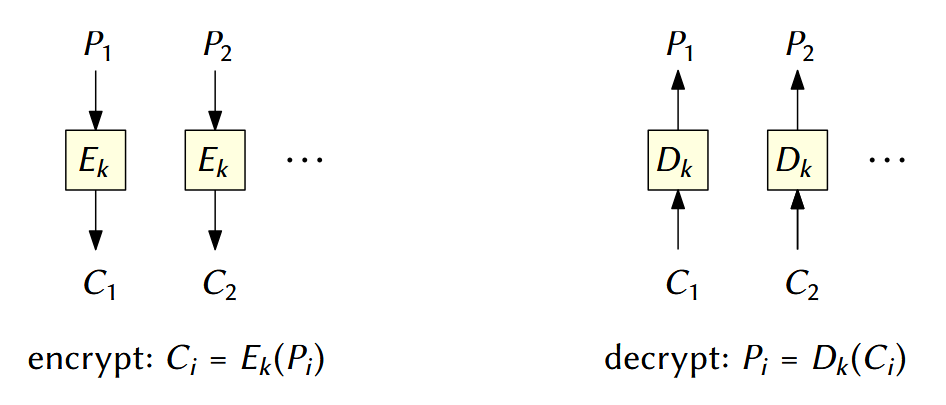
\includegraphics[width=\textwidth]{ecb.png}
                    \caption{ECB}
                    \label{fig:sub1}
                \end{subfigure}
                % Subfigure 2
                \begin{subfigure}[b]{0.4\textwidth}
                    \centering
                    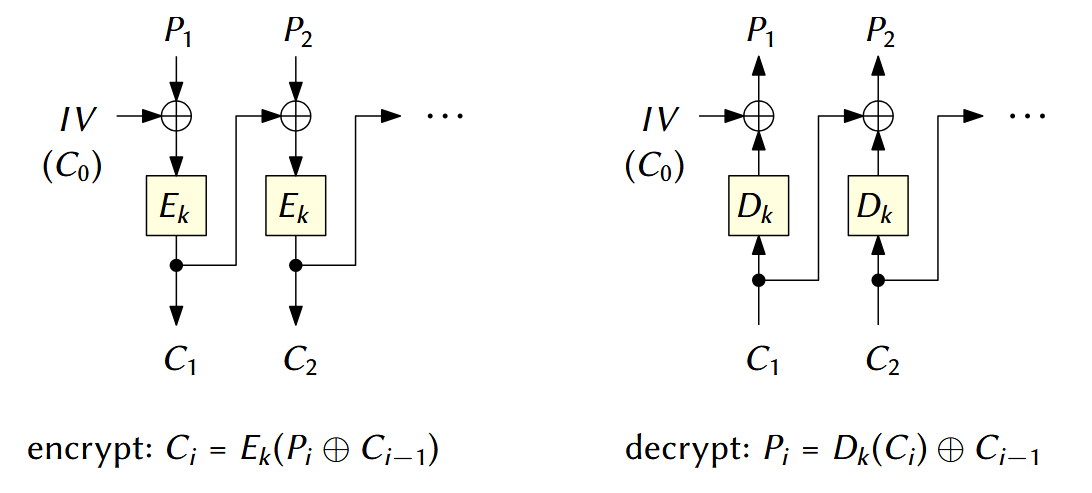
\includegraphics[width=\textwidth]{cbc.png}
                    \caption{CBC}
                    \label{fig:sub2}
                \end{subfigure}
                % Subfigure 3
                \begin{subfigure}[b]{0.4\textwidth}
                    \centering
                    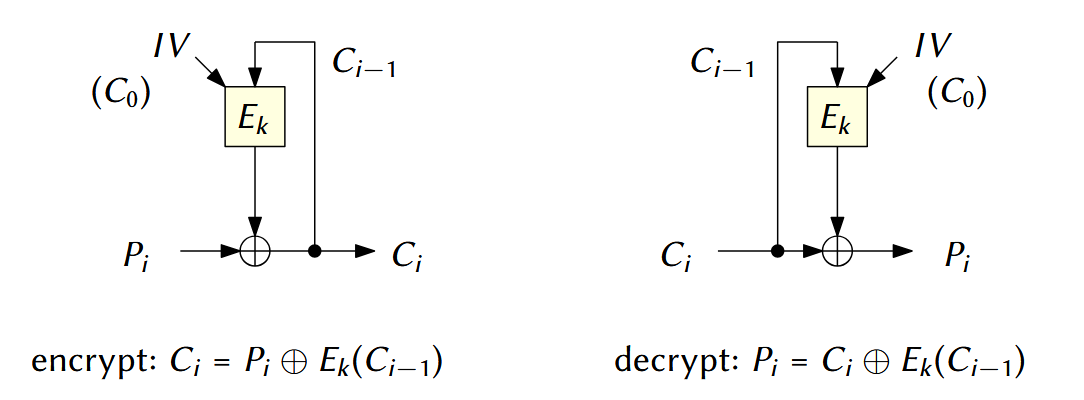
\includegraphics[width=\textwidth]{cfb.png}
                    \caption{CFB}
                    \label{fig:sub3}
                \end{subfigure}
                
                % Optional line break for next row
                \vspace{0.5cm}
            
                % Subfigure 4
                \begin{subfigure}[b]{0.4\textwidth}
                    \centering
                    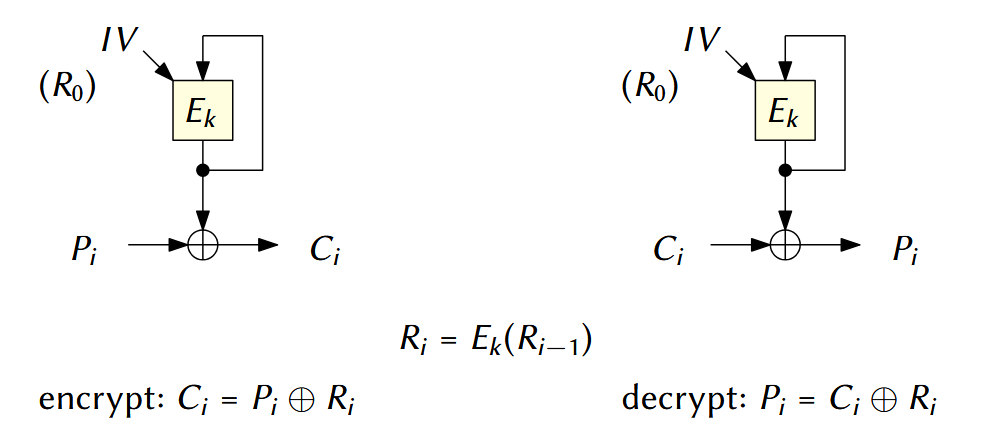
\includegraphics[width=\textwidth]{ofb.png}
                    \caption{OFB}
                    \label{fig:sub4}
                \end{subfigure}
                % Subfigure 5
                \begin{subfigure}[b]{0.4\textwidth}
                    \centering
                    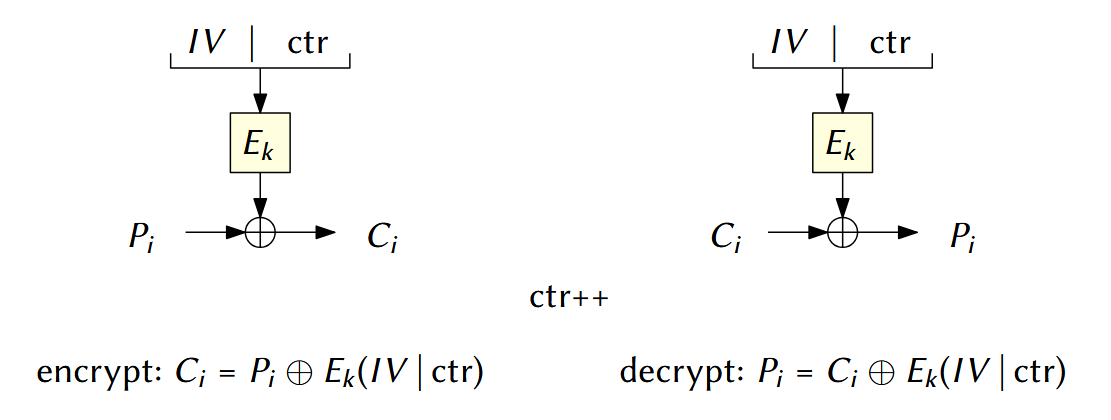
\includegraphics[width=\textwidth]{ctr.png}
                    \caption{CTR}
                    \label{fig:sub5}
                \end{subfigure}
            
                \caption{Módy zabezpečujúce len dôvernosť, nie autentickosť.}
                \label{fig:main}
            \end{figure}
            \item Ak správa nie je zarovnaná na násobok veľkosti bloku, je nutné použiť ciphertext stealing, resp. padding. Pri použití paddingu si treba dať pozor, aby sme nevytvorili zraniteľnosť.
        \end{itemize}
        \item Prúdové šifry šifrujú každý bit správy samostatne.
        \begin{itemize}
            \item Pomovou kľúča a inicializačného vektora (IV) sa inicializuje generátor pseudonáhodnej postupnosti bitov. Šifrový text je XOR otvoreného textu a generovanej postupnosti.
            \item Správa môže mať ľubovoľnú dĺžku.
        \end{itemize}
        \item Asymetrické šifry (viac detailov).
        \begin{itemize}
            \item Ich bezpečnosť je založená na ťažkých problémoch, napr. faktorizácia veľkých čísel alebo diskrétny logaritmus. Pri dostatočne silnom kvantovom počítači sú oba problémy riešiteľné (Shorov algoritmus), treba sa obrátiť na postkvantovú kryptografiu. Tá využíva iné ťažké problémy (mriežky, kódovanie a pod.).
        \end{itemize}
    \end{itemize}
    \subsection{Správa kryptografických kľúčov}
}

\examquestion{Integrita a autentickosť údajov}{
    \subsection{Motivácia, ciele, hrozby, príklady zraniteľností}
    \subsection{Integrita a autentickosť pri prenose a uložení údajov}
    \begin{itemize}
        \item Bezpečnostné požiadavky:
        \begin{itemize}
            \item Integrita -- údaje nie je možné zmeniť bez toho, aby to ich vlastník alebo adresát nemohol zistiť.
            \item Autentickosť -- deklarovaná identita autora, resp. odosielateľa údajov je pravdivá.
            \item Autentickosť je ``nadmnožinou'' integrity -- vieme, že údaje neboli zmenené a navyše vieme, kto ich zapísal. O úroveň vyššie je nepopretie autorstva.
        \end{itemize}
        \item Hash funkcie\label{hash}
        \begin{itemize}
            \item Funkcia $h:X\to Y$, ktorá deterministicky a efektívne (rýchlo) vypočíta odtlačok pevnej dĺžky $y=h(x)\in Y$ zo vstupu (skoro) ľubovoľnej dĺžky $x\in X$.
            \item Má vlastnosti:
            \begin{itemize}
                \item Pre-image resistance: pre $y=h(x)$ je ťažké nájsť $x$
                \item Second pre-image resistance: pre $x$ je ťažké nájsť $x'\neq x$ také, že $h(x)=h(x')$
                \item Collision resistance: je ťažké nájsť $x$ a $x'$ také, že $x\neq x'$ a $h(x)=h(x')$
            \end{itemize}
            \item TODO maybe birthday attack, constructions (hard problem, block cipher, Merkle-Damgard, Keccak, real examples)
        \end{itemize}
    \end{itemize}
    \subsection{Integrita v počítačových sieťach (CRC, v bezpečnostných protokoloch a pod.)}
    \begin{itemize}
        \item CRC
        \begin{itemize}
            \item CRC je cyklický kód, ktorý sa často používa na detekciu chýb pri prenose po počítačovej siete. Využíva sa napríklad v Etherntových rámcoch.
            \item 
        \end{itemize}
        \item IPsec -- AH, ESP voliteľne (dôležité detaily)
        \begin{itemize}
            \item Dva módy:
            \begin{itemize}
                \item Transportný -- AH/ESP hlavička sa vkladá medzi IP hlavičku a hlavičku transportnej vrstvy.
                \item Tunelový -- pôvodný paket sa ``zabalí'' do nového, ktorý má novú IP aj IPsec hlavičku, znova buď AH alebo ESP. Nový paket môže mať iné IP adresy, vhodné pri site-to-site VPN.
            \end{itemize}
            \begin{figure}[htbp]
              \centering
              \begin{subfigure}[b]{0.7\textwidth}
                \centering
                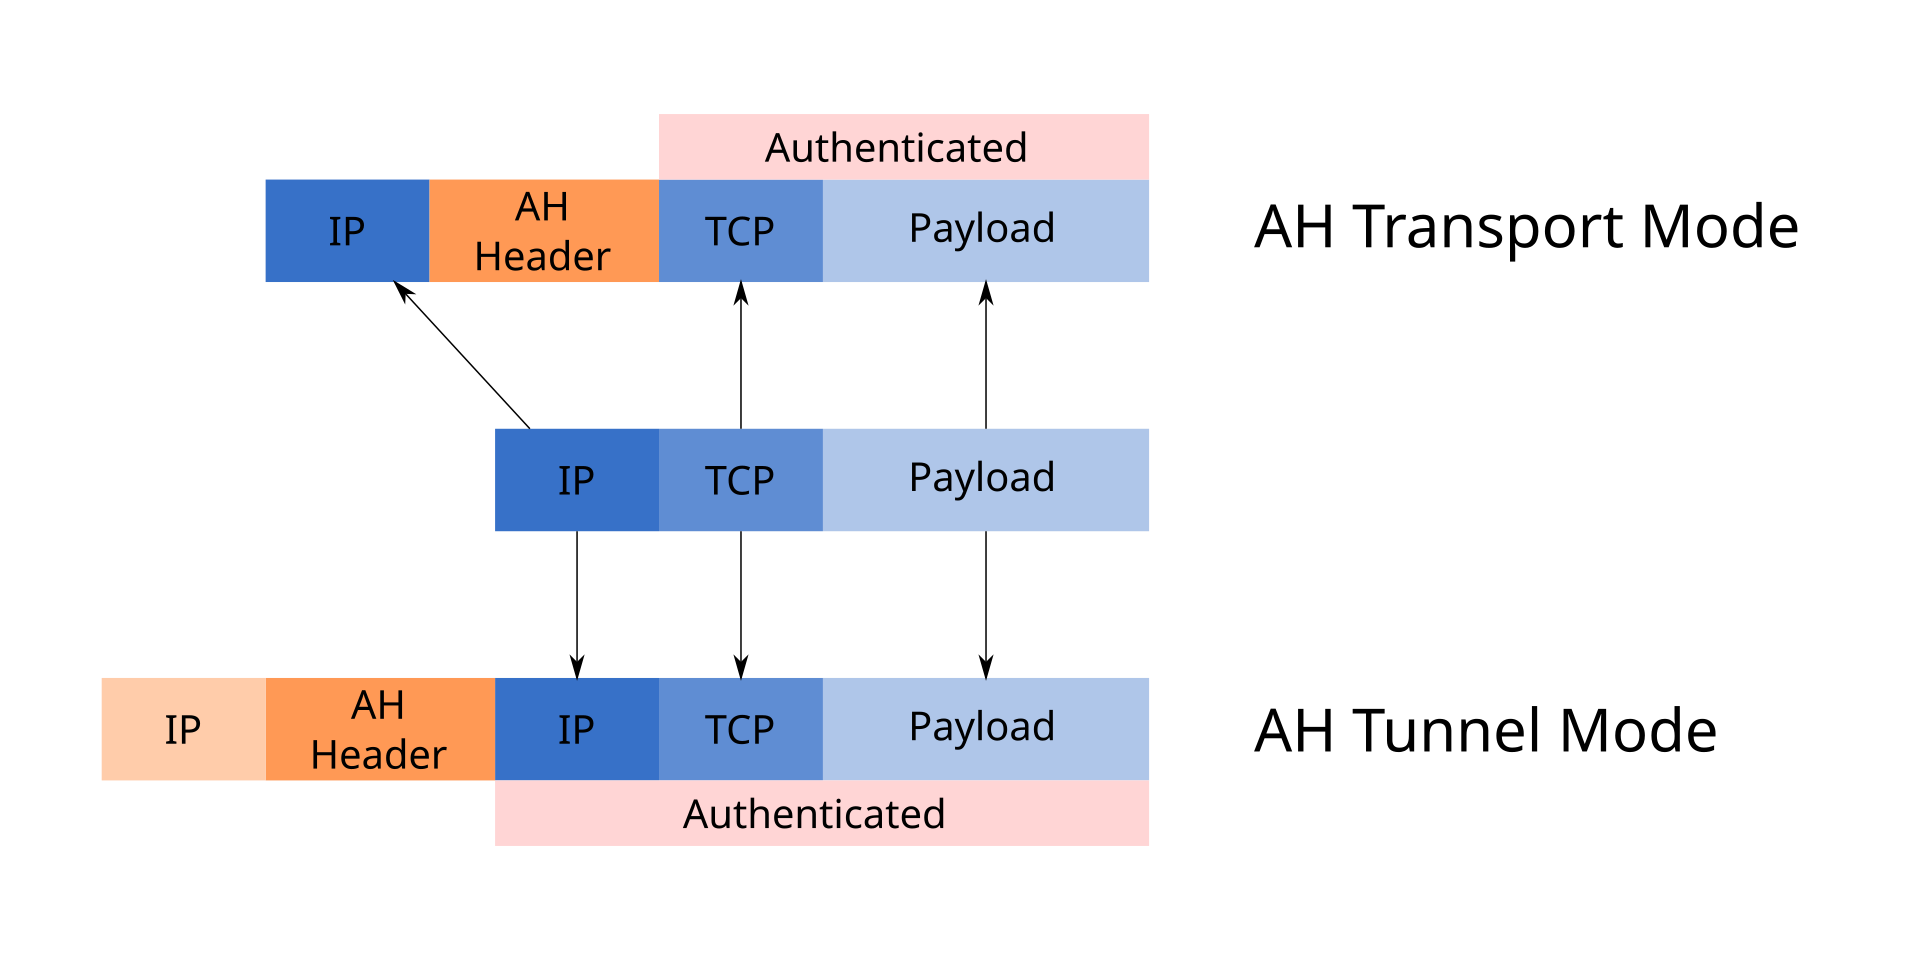
\includegraphics[width=\textwidth]{Ipsec-ah.svg.png}
                \label{fig:image1}
              \end{subfigure}
              \hfill
              \begin{subfigure}[b]{0.8\textwidth}
                \centering
                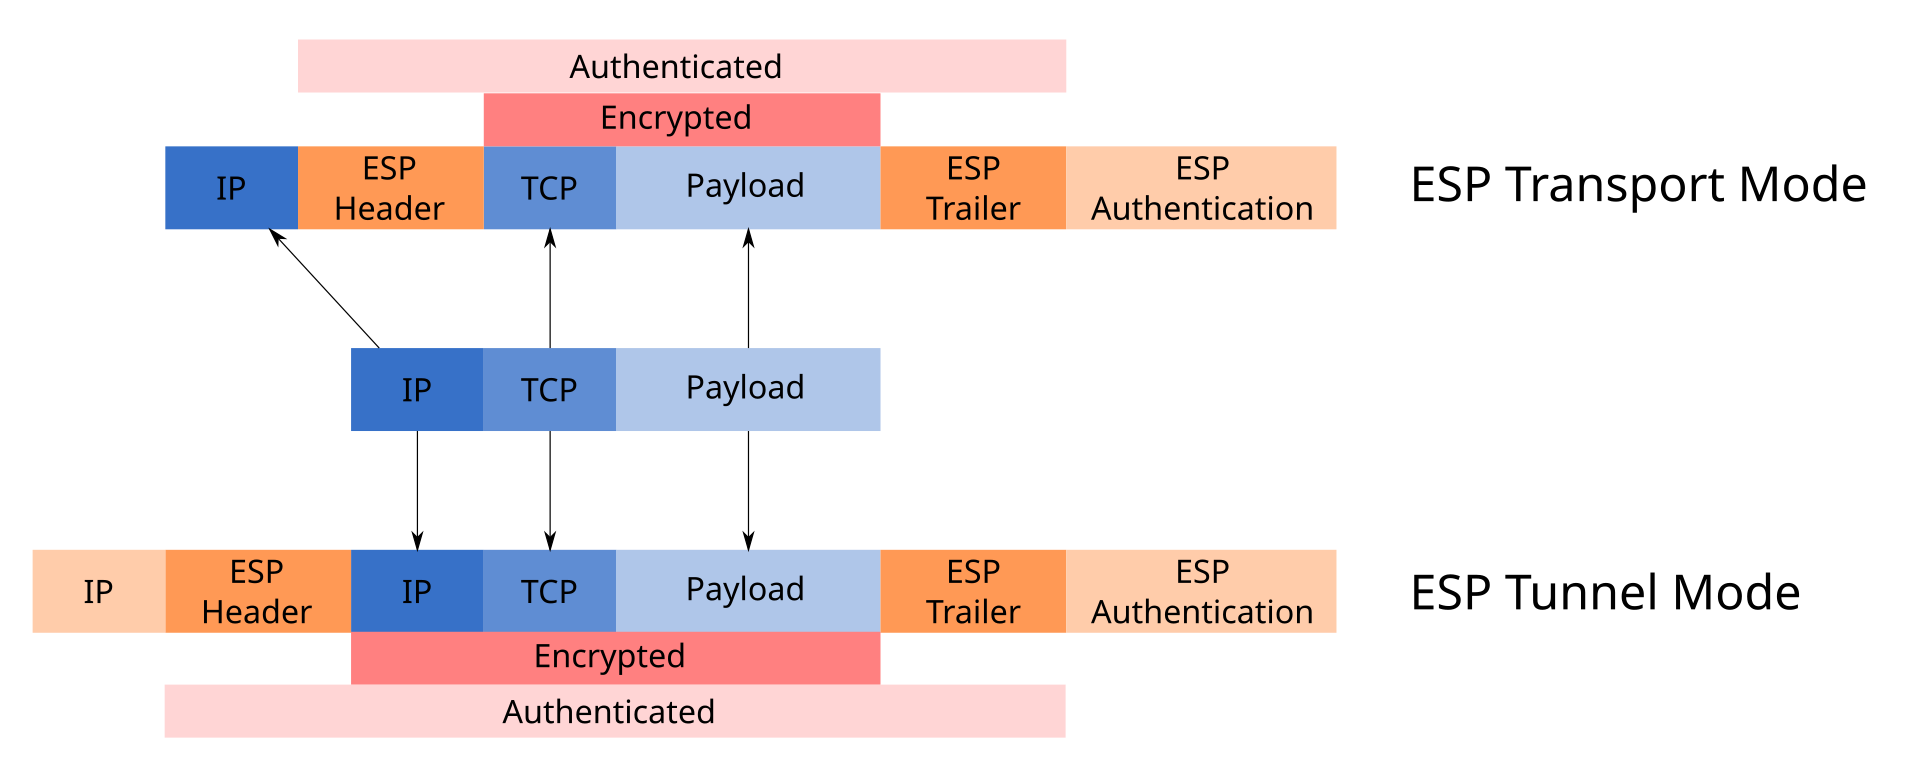
\includegraphics[width=\textwidth]{Ipsec-esp-tunnel-and-transport.svg.png}
                \label{fig:image2}
              \end{subfigure}
              \caption{Tunelový a transportný mód pre AH a ESP}
              \label{fig:combined}
            \end{figure}
            \item Authentication header (AH)
            \begin{itemize}
                \item Ochrana integrity -- nemenné časti IP hlavičky (pravdepodobne napr. TTL) pred AH, samotný AH (okrem políčka s checksum-om) a údaje transportnej a vyšších vrstiev.\footnote{Čo a ako sa presne nuluje sa dá pozrieť v Linux implementácii AH \href{https://github.com/torvalds/linux/blob/master/net/ipv4/ah4.c}{tu}.}
                \begin{figure}
                    \centering
                    \begin{bytefield}[bitwidth=1.1em]{32}
                        \bitheader{0-31} \\
                        \bitbox{4}{Version}
                        \bitbox{4}{IHL}
                        \bitbox{6}[bgcolor=highlight]{DSCP}
                        \bitbox{2}[bgcolor=highlight]{ECN}
                        \bitbox{16}[bgcolor=highlight]{Total length}\\
                        \bitbox{16}{Identification}
                        \bitbox{3}[bgcolor=highlight]{Flags}
                        \bitbox{13}[bgcolor=highlight]{Fragment offset}\\
                        \bitbox{8}[bgcolor=highlight]{Time to live}
                        \bitbox{8}{Protocol}
                        \bitbox{16}{Header checksum}\\
                        \bitbox{32}{Source address}\\
                        \bitbox{32}{Destination address}\\
                    \end{bytefield}
                    \caption{IPv4 hlavička, zvýraznené časti sa môžu meniť. ECN a DSCP môžu modifikovať routre po ceste, TTL nutne klesá, Total length, Fragment offset a Flags sa môžu zmeniť pri fragmentácii. Pri výpočte ICV sa hodnoty nahradia nulami.}
                    \label{fig:ipv4_header}
                \end{figure}
                \item Ochrana proti replay útoku -- sekvenčné číslo v hlavičke.
                \begin{figure}
                    \centering
                    \begin{bytefield}[bitwidth=1.1em]{32}
                        \bitheader{0-31} \\
                        \bitbox{8}{Next header}
                        \bitbox{8}{Payload len}
                        \bitbox{16}[bgcolor=highlight]{Reserved}\\
                        \bitbox{32}{Security parameters index}\\
                        \bitbox{32}{Sequence number}\\
                        \wordbox{2}[bgcolor=highlight]{Integrity check value \\ $\vdots$}
                    \end{bytefield}
                    \caption{AH hlavička, zvýraznené časti nie sú zahrnuté pri výpočte ICV.}
                    \label{fig:ah_header}
                \end{figure}
            \end{itemize}
            \item Encapsulating security payload (ESP)
            \begin{itemize}
                \item Ochrana integrity -- transportná vrstva a vyššie (transportný mód) alebo celý pôvodný paket (tunelový mód).
                \item Ochrana proti replay útoku -- sekvenčné číslo.
                \item TODO, dokončiť celé a skontrolovať
                \begin{figure}
                    \centering
                    \begin{bytefield}[bitwidth=1.1em]{32}
                      \bitbox{32}{Security parameters index}\\
                      \bitbox{32}{Sequence number}\\
                      \wordbox{1}[bgcolor=shade]{Payload data}\\
                      \bitbox[tlr]{32}[bgcolor=shade]{Padding}\\
                      \bitbox[l]{16}[bgcolor=shade]{}
                      \bitbox{8}{Pad length}
                      \bitbox{8}{Next header}\\
                      \wordbox{2}[bgcolor=highlight]{Integrity check value \\ $\vdots$}
                    \end{bytefield}
                    \caption{ESP hlavička a trailer. Šedé časti nie sú súčasťou ESP.}
                    \label{fig:esp_header}
                \end{figure}
            \end{itemize}
        \end{itemize}
        \item TCP/UDP -- checksumy v headeroch
        \item TLS -- HMAC alebo podpisy
        \item optionally DNSSEC, SSH
    \end{itemize}
    \subsection{Kryptografické metódy zabezpečenia autentickosti údajov (podpisové schémy, MAC a pod.)}
    \begin{itemize}
        \item Podpisové schémy
        \begin{itemize}
            \item Zabezpečujú integritu, autentickosť a nepopretie autorstva údajov. Okrem samotnej kryptografie sú na splnenie cieľov nutné PKI a legislatíva.
            \item Asymetrická konštrukcia -- na podpis sa používa súkromný kľúč, na overenie verejný. Na dôveryhodné šírenie verejného kľúča sa využíva PKI.
            \item Samotná schéma pozostáva z troch komponentov: (Gen, Sig, Vrf)
            \begin{itemize}
                \item Gen -- PPT\footnote{PPT (probabilistic polynomial-time) algoritmus je znáhodnený a beží v polynomiálnom čase.} algoritmus na generovanie páru kľúčov (verejný a súkromný).
                \item Sig -- PPT algoritmus na podpísanie údajov, vstupom sú údaje a súkromný kľúč podpisujúceho.
                \item Vrf -- PT (deterministický) algoritmus na overenie podpisu, vstupom je podpis, údaje a podpisujúceho verejný kľúč.
            \end{itemize}
            \item V korektnej schéme pre každú dvojicu kľúčov a ľubovoľnú správu platí, že overenie podpisu skončí úspešne. TODO matematický zápis.
            \item EUF-CMA bezpečnosť.
            \item RSA, paddingy, ElGamal, DSA, ECDSA, Schnorr, EdDSA
        \end{itemize}
    \end{itemize}
}

\examquestion{Elektronický podpis, PKI a ich aplikácie}{
    \subsection{Vlastnoručný podpis ako bezpečnostná funkcia}
    \begin{itemize}
        \item Funkcia vlastnoručného podpisu -- vyjadrenie súhlasu podpísanej osoby s obsahom dokumentu.
        \item Takýto podpis je (ideálne):
        \begin{itemize}
            \item nefalšovateľný
            \item neprenositeľný na iný dokument
            \item je možné zistiť dodatočnú zmenu obsahu dokumentu
            \item identifikovať podpisovateľa
        \end{itemize}
    \end{itemize}
    \subsection{Elektronický podpis. Implementácia elektronického podpisu pomocou digitálneho. Vytváranie a overovanie elektronických podpisov}
    \begin{itemize}
        \item Elektronický podpis je všeobecný pojem z direktívy EÚ, digitálny podpis je kryptologický prostriedok využívaný na realizáciu elektronických podpisov.
        \item Definícia dokumentu
        \begin{itemize}
            \item informačný obsah (zaznamenaný v podobe údajov)
            \item formát (konvencia ako interpretovať údaje)
            \item bezpečnostné mechanizmy (ochranné prvky na zaistenie CIA, príp. iných požiadaviek)
            \item úroveň bezpečnostných záruk (odvíja sa od výberu mechanizmov a ich parametrov, mapr. dĺžka kľúčov)
            \item realizácia (papierový, súbor uložený v pamäti, prenášaný komunikačným kanálom prostredníctvom signálov a pod.)
        \end{itemize}
        \item Na implementáciu digitálneho podpisu využívame asymentrický kryptosystém -- šifrujeme obsah dokumentu\footnote{Štandardne sa šifruje kryptografický hash obsahu, keďže šifrovaný plaintext nemôže byť ľubovoľne dlhý a asymetrické konštrukcie sú výpočtovo náročné. Takýto hash sa vytvára pomocou kryptografickej hash funkcie popísanej v \ref{hash}.} (podpisujeme) pomocou súkromného kľúča a dešifrujeme (overujeme) pomocou verejného. Namiesto dôvernosti takto zabezpečujeme integritu a autentickosť. 
        \item Kryptografická konštrukcia (hash + asymetrická šifra) a utajenie (zverejnenie) súkromného (verejného) kľúča  zabezpečujú nefalšovateľnosť\footnote{Pre pospisové schémy sa dokazuje EUF-CMA bezpečnosť, t.j. za určitých dostatočných predpokladov dokáže vytvoriť platný podpis len ten, kto pozná súkromný kľúč.}, neprenositeľnosť na iný dokument\footnote{Vyplýva zo second pre-image resistance hash funkcie.} a umožňujé zistiť dodatočnú zmenu obsahu dokumentu\footnote{Vyplýva z collision resistance hash funkcie.}.
        \item Je nutné ešte zaistiť bezpečnú (dôveryhodnú) distrubúciu verejných kľúčov, ktorá umožní identifikáciu podpisovateľa. Toto zabezpečíme pomocou certifikátov a PKI.
    \end{itemize}
    \subsection{Certifikát verejného kľúča (význam, hlavné položky a ich význam). Rušenie certifikátov, zoznam zrušených certifikátov. Časové pečiatky. Elektronická pečať}
    \begin{itemize}
        \item Certifikát verejného kľúča -- elektronický dokument, ktorým jeho vydavateľ potvrdzuje, že v certifikáte uvedený verejný kľúč patrí osobe (príp. inému subjektu), ktorej identifikačné údaje (meno) sú tiež v certifikáte uvedené (držiteľ certifikátu).
        \begin{itemize}
            \item Certifikát vydáva dôveryhodná tretia strana -- certifikačná autorita.
            \item Formát je upravený štandardom X509.
            \item Obsahuje:\footnote{Modrá označuje prvky nutné pre overenie autentickosti certifikátu a červená prvky plniace jeho hlavný účel -- zviazanie identity a verejného kľúča.}
            \begin{itemize}
                \item \textcolor{black}{identifikačné číslo certifikátu}
                \item \textcolor{blue}{identifikačné údaje vydavateľa certifikátu}
                \item \textcolor{red}{identifikačné údaje držiteľa certifikátu}
                \item dátum a čas začiatku a konca platnosti certifikátu
                \item \textcolor{red}{verejný kľúč držiteľa certifikátu}
                \item identifikáciu algoritmov, pre ktoré je kľúč určený
                \item \textcolor{blue}{elektronický podpis certifikačnej autority}
            \end{itemize}
        \end{itemize}
        \item V prípade prezradenia alebo straty súkromného kľúča je nutné zrušiť (revokovať) certifikát, aby sa predišlo problémom.
        \item Rušenie certifikátu realizuje certifikačná autorita jeho zaradením do Certificate revocation list (CRL). Je to elektronický dokument, ktorým CA oznamuje predčasné skončenie platnosti certifikátu. Obsahuje tieto položky:
        \begin{itemize}
            \item identifikačné údaje CA
            \item dátum a čas vydania CRL
            \item dátum a čas najneskoršieho vydania nového CRL
            \item zoznam identifikačných čísel zrušených certifikátov
            \item elektronický podpis certifikačnej autority
        \end{itemize}
        \item Pri overení podpisu je teraz nutné okrem iného skontrolovať, či sa certifikát nenachádzal v CRL v čase vytvorenia podpisu.
        \begin{itemize}
            \item Bez tohoto kroku by boli možné podvody. Napríklad Alica by mohla podpísať zmluvu, poslať ju Bobovi, zrušiť svoj certifikát a vyhlásiť zmluvu za neplatnú. 
        \end{itemize}
        \item Časové pečiatky plnia funkciu objektívneho časového údaju viazaného na dokument.
        \item Pečiatky vydáva CA, resp. iný dôveryhodný poskytovateľ. Pečiatka pozostáva a hashu podpisovaného dokumentu a času, ktoré sú autoritou podpísané.
        \begin{itemize}
            \item Bob pred akceptovaním zmluvy požiada o vydanie pečiatky. Ak by sa teraz Alica pokúsila o podvod, bola by časová pečiatka podpisu je skoršia ako čas v CRL, čiže podpis je platný.
        \end{itemize}
        \item Elektronická pečať podpisuje dokument za organizáciu (právnická osoba), zaručuje pôvod a integritu. Technicky sa jedná o certifikát verejného kľúča, rozdiel je právny, resp. sémantický (TODO overiť). Viac \href{https://snca.gov.sk/kvalifikovane-sluzby/elektronicka-pecat}{tu}.
    \end{itemize}
    \subsection{Certifikačná autorita. Koreňová certifikačná autorita, krížová certifikácia. Certifikačná cesta, certifikát verejného kľúča R-CA. \hl{Iné typy certifikátov (atribútové, mandátové a ich použitie)}}
    \begin{itemize}
        \item Certifikačná autorita je základom PKI. Jej úlohou je vydávanie a rušenie certifikátov, vydávanie CRL, zverejňovanie certifikátov, poskytovanie služby časových pečiatok atď.
        \item PKI môže maž dve architektúry -- hierarchická alebo mesh. 
        \item V hierarchickej je základom štruktúry koreňová CA. Jej úlohou je manažment certifikátor pre CA nižšej úrovne. Keďže je koreňová, svoj verejný kľúč si sama zverejňuje spolu so self-signed certifikátom. Tento certifikát je potom nutné rozšíriť bezpečnou fyzickou distribúciou, napr. operačné systémy štandardne obsahujú certifikáty viacerých známych koreňových CA. Na najnižšej úrovni sú CA, ktoré poskytujú certifikáty koncovým používateľom.
        \begin{itemize}
            \item Overenie certifikátu je rekurzívny algoritmus s konečným počtom krokov:
            \begin{itemize}
                \item Over podpis certifikátu A pomocou verejného kľúča CA z certifikátu B.
                \item Over platnosť a či nie je v CRL (prípadne OCSP\footnote{Online certificate status protocol (OCSP) je alternatívny spôsob overenia platnosti certifikátu. Pošleme dotaz OCSP responder s identifikačným číslom certifikátu a dostaneme späť podpísanú odpoveď \textit{good} alebo \textit{revoked}. Výhoda oproti CRL je, že nemusíme sťahovať a prehľadávať celý zoznam, no pri OCSP prichádzame o súkromie.}).
                \item Ak certifikát B patrí dôveryhodnej koreňovej CA, skonči. Inak pokračuj rekurzívne s certifikátom B.
            \end{itemize}
        \end{itemize}
        \begin{figure}[htbp]
            \centering
            \begin{tikzpicture}[
              cert/.style={draw, rounded corners, minimum width=3.5cm, minimum height=1.5cm, align=center},
              arrow/.style={->, thick}
            ]
            
            % Certifikáty
            \node[cert] (A) {Certifikát A \\ \footnotesize (Subjekt) \\ obsahuje Verejný kľúč A};
            \node[cert, right=5.8cm of A] (B) {Certifikát B \\ \footnotesize (Vydavateľ -- CA) \\ obsahuje Verejný kľúč B};
            
            % Šípka podpisu
            \draw[arrow] (B.west) -- node[above]{\footnotesize podpísaný Súkromným kľúčom B} (A.east);
            
            % Súkromné kľúče
            \node[below=1.3cm of A] (Apriv) {\footnotesize Súkromný kľúč A (tajný)};
            \node[below=1.3cm of B] (Bpriv) {\footnotesize Súkromný kľúč B (tajný)};
            
            % Spojenia
            \draw[dashed] (A.south) -- (Apriv.north);
            \draw[dashed] (B.south) -- (Bpriv.north);
            
            \end{tikzpicture}
            \caption{Krok na certifikačnej ceste.}
            \label{fig:placeholder}
        \end{figure}
        \item V architektúre typu mesh nie je koreňová autorita, každá CA má svoju doménu, kde pôsobí, a navzájom si vydávajú certifikáty (krížová certifikácia). Takto je možné overiť certifikát koncového koncového používateľa z inej domény. 
        \begin{figure}[htbp]
            \centering
            % Subfigure 1
            \begin{subfigure}[b]{0.48\textwidth}
                \centering
                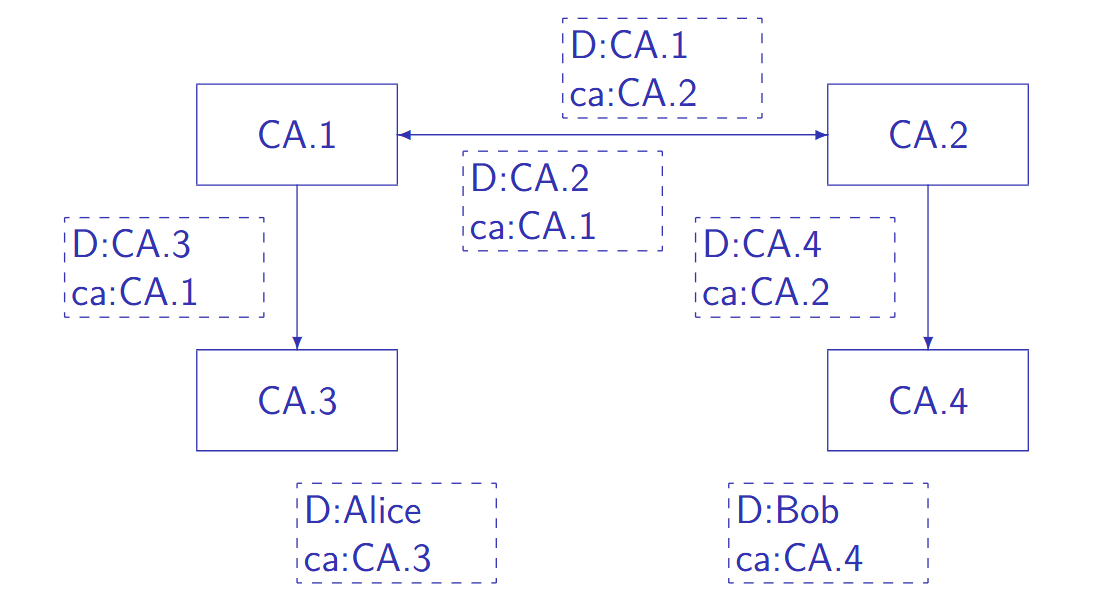
\includegraphics[width=\textwidth]{mesh_ca.png}
                \caption{Mesh}
                \label{fig:mesh}
            \end{subfigure}
            % Subfigure 2
            \begin{subfigure}[b]{0.48\textwidth}
                \centering
                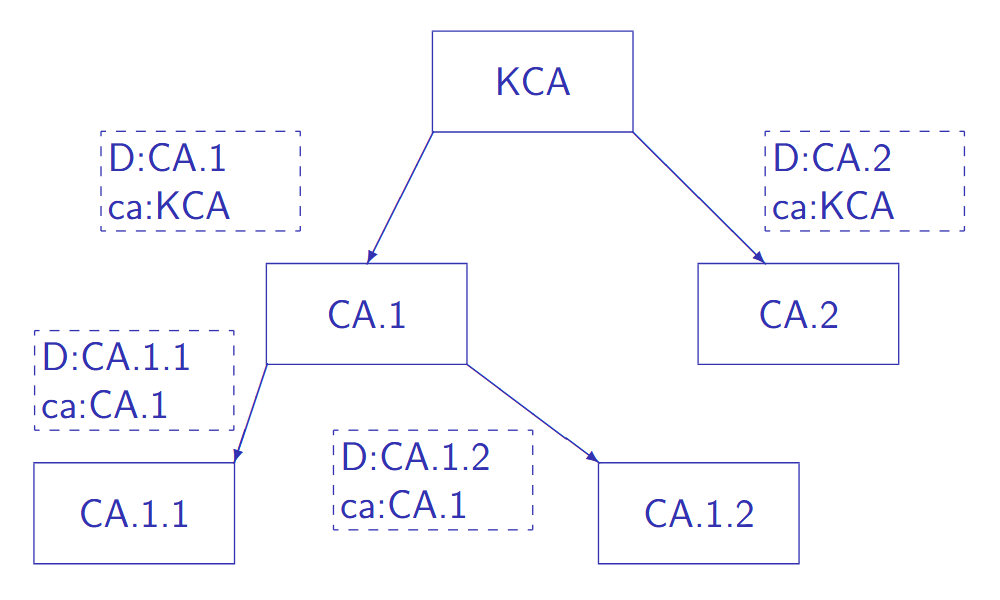
\includegraphics[width=\textwidth]{root_ca.png}
                \caption{Hierarchická}
                \label{fig:root}
            \end{subfigure}        
            \caption{Architektúry PKI.}
            \label{fig:main}
        \end{figure}
        \item Atribútový certifikát (AC) viaže atribúty alebo rolu k držiteľovi (teda namiesto kľúča viaže atribúty k identite), tie mu udelil vydavateľ certifikátu. Viac \href{https://en.wikipedia.org/wiki/Authorization_certificate}{tu}.
        \item Mandátový certifikát je špeciálny AC, deleguje právomoc jednej entite konať v mene inej. Viac \href{https://snca.gov.sk/kvalifikovane-sluzby/mandatny-certifikat}{tu}. TODO rozpísať tieto dva body.
    \end{itemize}
    
}

\examquestion{Dostupnosť}{
    \subsection{Motivácia, ciele, hrozby, príklady zraniteľností; dostupnosť služieb a dostupnosť dát}
    \begin{itemize}
    \item Požiadavka, aby zdroje systému boli k dispozícii oprávnenej osobe 
    \begin{enumerate}
        \item Vždy keď o to požiada,
        \item do času $t$ od okamihu, keď o to požiada,
        \item s pravdepodobnosťou meranou podielom doby, keď sú požadované zdroje k dispozícii ku celkovej dobe.
    \end{enumerate}
        \item Technické zlyhania, požiar, záplavy, krádež, úmyselné, resp. neúmyselné zmazanie dát a pod. sú hrozby, ktoré môžu obmedziť dostupnosť dát.
        \item Pre rôzne hrozby existujú účinné opatrenia. Patria medzi ne napr. zálohovanie, RAID, záložné datacentrá v iných lokalitách, riadenia prístupu. Opatrenia majú rôznu úspešnosť podľa toho akej hrozbe čelíme.
        
    \end{itemize}
    \subsection{Dostupnosť pri výpadku IT komponentov (failover) a dostupnosť pri záťaži (rozkladanie záťaže)}
    \begin{itemize}
        \item Failover je mechanizmus, ktorý automaticky uvedie do prevádzky záložný komponent pri výpadku primárneho.
        \item Rozkladanie záťaže je proces distribuovania pricádzajúcej sieťovej prevádzky, požiadaviek alebo výpočtových úloh medzi viaceré komponenty. Účel je optimalizácia výkonu alebo maximalizácia priepustnosti systému.
        \item Máme dve rovnocenné komponenty, jeden primárny a jeden sekundárny. Pri bežnej prevádzke sa používa primárny komponent. V prípade poruchy preberie jeho úlohu sekundárny komponent.
    \end{itemize}
    \subsection{Podpora pre zvýšenie dostupnosti v sieťových protokoloch: smerovanie, DNS, Anycast a pod.}
    \begin{itemize}
        \item OSPF -- loadbalancing resp. automatické presmerovanie prevázdky cez alternatívnu linku pri výpadku primárnej.
        \item BGP -- dovoľuje alternatívne linky (asi? treba pozrieť).
        \item DNS -- 
        \item anycast -- viacero zariadení zdieľa tú istú, tzv. anycast-ovú, adresu, routre pošlú prevádzky k najbližšiemu. Využitie pri CDN alebo root DNS serveroch (Existuje 13 adries, t.j. servery a až m, za každou sa ale ``skrýva'' veľa serverov). Toto by nebolo zlé si pozrieť ešte viac.
        \item STP
        \begin{itemize}
            \item Vzhľadom na princíp fungovania Ethernetu je nutné zabezpečiť, aby v takejto sieti neexistovali slučky (vznikne broadcast storm). Nie je teda možné mať viacero alternatívnych liniek medzi switchmi, čo vytvára SPOF a predstavuje ohrozenie dostupnosti. 
            \item Protokol STP redundantné linky medzi switchmi vypne, čím zamedzí vzniku slučiek. V prípdade výpadku linky niektorú z redundantných sfunkční. Ak máme dostatočne veľa redundantných liniek, vieme takto ``prežiť'' aj výpadok switcha.
        \end{itemize}
        \item možno okrajovo veci ako load balancery, FHRP, availability zóny v cloude
    \end{itemize}
    \subsection{Zálohovanie, RAID, klastre a pod.}
    \subsection{Havarijné plány a plány obnovy činnosti}
}

\examquestion{Klasifikácia informácie a systémov}{
    \subsection{Zmysel a podstata klasifikácie. Kritériá klasifikácie informácie (CIAA)}
    \begin{itemize}
        \item Confidentiality (dôvernosť) --
    \end{itemize}
    \subsection{Klasifikácia informácie. Klasifikácia systémov}
    \subsection{Kategórie opatrení. Súbory opatrení pre jednotlivé triedy systémov. Metodika BSI Grundschutz}
    \begin{itemize}
        \item Opatrenia delíme do kategórií podľa použitých prostriedkov a v ktorej ``fáze incidentu'' pôsobia

        \begin{table}[htbp]
            \centering
            \begin{tabular}{|l|p{11cm}|}
              \hline
              Preventívne &
              \footnotesize
              Zamedzujú vzniku bezpečnostného incidentu, teda môžu:
              \begin{itemize}\setlength\itemsep{0pt}
                \item odstrániť zraniteľnosť
                \item zvýšiť pravdepodobnosť odhalenia (znižuje motiváciu)
                \item obmedziť príležitosti
                \item zvýšiť potrebnú úroveň znalostí útočníka\footnote{Motivácia, príležitosť a znalosti spolu tvoria útočný potenciál.}
              \end{itemize} \\ \hline
              Detekčné & Včas odhalia začínajúci incident a umožnia včasnú reakciu, sú to napr. čidlo na dym alebo pohyb, IDS, monitorovací softvér a pod.\\ \hline
              Korekčné & Zamerané na zabezpečenie kontinuity činnosti, teda pomáhajú riešiť vzniknutý incident a vrátiť aktívum do normálneho stavu. Sú to napr. TODO\\ \hline
            \end{tabular}
        \end{table}   


        \begin{table}[htbp]
            \centering
            \begin{tabular}{|l|p{11cm}|}
              \hline
              Technické    & Bezpečnostné funkcie realizované hardvérom alebo softvérom.\\ \hline
              Organizačné  & Nastavenie politík, pravidiel, postupov, zodpovednosti, školení a zmlúv.\\ \hline
              Prevádzkové  & Fyzická ochrana IKT a podpornej infraštruktúry. \\ \hline
            \end{tabular}
        \end{table}
    \end{itemize}
}

\examquestion{Systém riadenia informačnej bezpečnosti (ISMS)}{
    \begin{itemize}
        \item Information Security Management System
        \item Virtuálny systém pozostávajúci z:
        \begin{itemize}
            \item princípov riadenia KIB
            \item zdroje, ktoré sú na zaistenie a udržiavanie KIB potrebné
            \item ľudí, ktorí pracujú s informáciami, systémami a sieťami a plnia buď špeciálne úlohy v KIB alebo zohľadňujú KIB pri plnení svojich pracovných úloh
            \item bezpečnostného procesu (aktivity zamerané na dosiahnutie a udržanie potrebnej úrovne KIB v organizácii)
            \begin{itemize}
                \item úlohou vedenia organizácie je tento proces iniciovať a riadiť
            \end{itemize}
        \end{itemize}
        \item Založený na formálne zdokumentovaných a koordinovaných bezpečnostných politikách, ktoré:
        \begin{itemize}
            \item Stanovujú ciele a úroveň informačnej bezpečnosti
            \item Určujú zodpovednosti za informačnú bezpečnosť (IB)
            \item Definujú organizačné zabezpečenie bezpečnosti
            \item Upravujú požiadavky na:
            \begin{itemize}
                \item Personálnu bezpečnosť (napr. školenia, kontroly zamestnancov)
                \item Vzťahy s externými partnermi (napr. zmluvy, dôvernosť údajov)
                \item Fyzickú bezpečnosť (napr. prístup do budov, zamknuté priestory)
                \item Prevádzkovú a komunikačnú bezpečnosť (napr. sieťová ochrana, logovanie)
                \item Ochranu prístupu (napr. prístupové práva, autentifikácia)
                \item Súlad s legislatívou (napr. GDPR, zákony o kybernetickej bezpečnosti)
            \end{itemize}
        \end{itemize}
    \end{itemize}
    \subsection{Motivácia, legislatívne požiadavky, medzinárodné a domáce štandardy}
    \begin{itemize}
        \item Slovenská legislatíva:
        \begin{itemize}
            \item Zákon č. 69/2018 Z. z. o kybernetickej bezpečnosti a o zmene a doplnení niektorých zákonov (v znení neskorších predpisov)
            \item Vyhláška Národného bezpečnostného úradu, č. 362/2018 Z. z.
            \begin{itemize}
                \item ustanovuje obsah bezpečnostných opatrení, obsah a štruktúra bezpečnostnej dokumentácie a rozsah všeobecných bezpečnostných opatrení
            \end{itemize}
            \item Zákon č. 95/2019 Z. z. o informačných technológiách vo verejnej správe a o zmene a doplnení niektorých zákonov
            \item Vyhláška Úradu podpredsedu vlády Slovenskej republiky pre investície a informatizáciu č. 179/2020 Z. z.
            \begin{itemize}
                \item ustanovuje spôsob kategorizácie a obsah bezpečnostných opatrení informačných technológií verejnej správy
            \end{itemize}
        \end{itemize}
        \item Európska legislatíva:\footnote{Druhy európskych legislatívnych aktov: \begin{enumerate}
            \item Odporúčania -- nie je záväzné, umožňuje inštitúciam EÚ prezentovať svoje názory a navrhovať kroky.
            \item Smernice -- stanovuje cieľ, ktorý musia dosiahnuť všetky krajiny EÚ. Je na každej krajine ako cieľ implementujú vo vlastnej legislatíve.
            \item Nariadenia -- záväzná, automaticky sa uplatňuje vo všetkých členských štátoch. Nie je potrebné transponovať do vlastných predpisov ako tomu je pri smernici.
        \end{enumerate}}
        \begin{itemize}
            \item NIS2 -- Európska smernica o kybernetickej bezpečnosti
            \begin{itemize}
                \item stanovuje povinnosti pre organizácie v kľúčových a dôležitých odvetviach s cieľom zlepšiť ich ochranu pred kybernetickými hrozbami a zvýšiť odolnosť ich IT a komunikačných systémov
            \end{itemize}
            \item GDPR
            \item eIDAS
        \end{itemize}
        \item Štandardy:
        \begin{itemize}
            \item séria štandardov ISO 27000 TODO spracujme  \href{https://www.csirt.sk/prehlad-standardov-iso-iec-27000.html}{odtiaľto}
            \item BSI Grundschutz
        \end{itemize}
    \end{itemize}
    \subsection{Postup pri zavádzaní ISMS. Bezpečnostná politika (obsah, vypracovanie, správa). Bezpečnostné štandardy a praktiky}
    \begin{itemize}
        \item Proces iniciuje vedenie organizácie. Na začiatku musí formálne prijať zodpovednosť a zaviazať sa riešiť KIB.
        \item Úlohou vedenia je následne:
        \begin{itemize}
            \item iniciovať proces -- vymenovať zamestnancov zodpovedných za KIB, poskytnúť im oprávnenia a zdroje (zvyčajne títo zamestnanci vypracujú bezpečnostnú politiku, ktorú následne schvaľuje vedenie, následne sa pravidelne reviduje)
            \item monitorovať proces -- vedenie pravidelne dostáva informácie o stave KIB v organizácii, najmä informácie o možných rizikách vyplývajúcich z chýbajúcich alebo nedostatočných bezpečnostných opatrení
            \item riadiť proces -- aktívne sa doň zapájať, napr. TODO
        \end{itemize}
        \item Dôležitá funkcia je Manažér KIB. Je to výkonná funkcia, no výstupy jeho práce sú predmetom prerokovania a schválenia vedením organizácie. Úlohy manažéra sú:
        \begin{itemize}
            \item riadenie bezp. procesu
            \item pomáha vedeniu pri tvorbe a správe bezp. politiky
            \item vypracováva podklady pre vedenie (napr. prehľad o stave KIB)
            \item vyšetruje bezp. incidenty
            \item a iné
        \end{itemize}
        \item Bezpečnostná politika je formálny dokument:
        \begin{itemize}
            \item schválený vedením inštitúcie
            \item podrobnejšie rozpracováva bezpečnostné ciele inštitúcie
            \item upresňuje úroveň bezpečnostných požiadaviek
            \item stanovuje zodpovednosť za informačnú bezpečnosť v organizácii
            \item rámcovo definuje spôsoby na dosiahnutie stanovených cieľov
        \end{itemize}
        \item Dokument sa odkazuje na \textit{bezpečnostné politiky 2. úrovne}, ktoré rozpracúvajú jendotlivé oblasti (napr. riadenie prístupu, fyzickú bezpečnosť, zálohovanie a pod.) 
    \end{itemize}
    \subsection{Analýza rizík, návrh opatrení, správa rizík. Bezpečnostné roly. Bezpečnostný manažment}
    \begin{itemize}
          \item Bezpečnostná politika ustanovuje kontext:
          \begin{itemize}
            \item Celkové bezpečnostné ciele a princípy
            \item Akceptovateľnú úroveň rizika (mieru rizikovej tolerancie)
            \item Prístup k riadeniu rizík (metodiku hodnotenia rizík)
            \item Zodpovednosti a účtovnú zodpovednosť (napr. vlastníci aktív, schvaľovatelia rizík)
            \item Odkazy na právne, regulačné a zmluvné požiadavky
          \end{itemize}
          
          \item Identifikácia rizík zahŕňa:
          \begin{itemize}
            \item Zmapovanie aktív organizácie a určenie vlastníkov aktív
            \item Identifikáciu relevantných hrozieb a zraniteľností
            \item Zaznamenanie existujúcich bezpečnostných opatrení
            \item Posúdenie požadovanej úrovne ochrany každého aktíva
                  (napr. dôvernosť, integrita, dostupnosť)
          \end{itemize}
        % \item Máme stanovenú akceptovateľnú hranicu rizika (bezp. politika)
        % \item Potrebujeme teraz vyhodnotiť čo chceme chrániť pred čím a na akej úrovni.
        % \begin{itemize}
        %     \item čo -- potrebujeme mať zmapované aké aktíva máme v organizácii a kto je ich vlastník (zodpovedný za aktívum)
        %     \item pred čím -- vrámci analýzy identifikujeme relevantné hrozby voči aktívam a existujúce bezp. opatrenia
        %     \item na akej úrovni -- vyplýva z bezp. politiky a špecifických požiadaviek (vyplývajú napr. z právnych predpisov, zmlúv a pod.)
        % \end{itemize}
        \item Výpočet hodnoty rizika
        \begin{itemize}
            \item Riziko zohľadňuje dopad (vážnosť) hrozby a jej pravdepodobnosť.
            \item Môžeme použiť kvantitatívny prístup (napr. $riziko=pravdepodobnosť*dopad$) alebo kvalitatívny (hodnotenie na škále nízké -- stredné -- vysoké)
            \item Organizácia by mala mať vytvorené kritériá na hodnotenie dopadu hrozby, napr. podľa úrovne klasifikácie postihnutých aktív, finančných strát, narušenia činností alebo plánov, porušenia právnych požiadaviek a pod.
        \end{itemize}
        \item Ak hodnota rizika prekračuje akceptovateľnú hodnotu, je nutné ho ošetriť:
        \begin{itemize}
            \item redukcia rizika -- prijatie technických, organizačných, personálnych a pod. opatrení ktoré znižujú pravdepodobnosť alebo dopad hrozby pod úroveň akceptovateľného rizika
            \item vyhnutie sa riziku -- zmena podmienok, ktoré viedli k vysokej hodnote rizika, napr. činnosť vykonávame iným spôsobom, v inom (menej nebezpečnom) prostredí
            \item prenesenie rizika -- riziko znáša subjekt, ktorý ho vie efektívnejšie riešiť, teda napr. poistenie, vyššia SLA\footnote{SLA=Service Level Agreement -- zmluva medzi zákazníkom a dodávateľom špecifikujúca o.i. napríklad garantovaný uptime, response time, resolution time, parametre ako throughput/latencia.}
        \end{itemize}
        \item Návrh opatrení 
        \begin{itemize}
            \item Opatrenia delíme do kategórií podľa použitých prostriedkov a v ktorej ``fáze incidentu'' pôsobia

        \begin{table}[htbp]
            \centering
            \begin{tabular}{|l|p{11cm}|}
              \hline
              Preventívne &
              \footnotesize
              Zamedzujú vzniku bezpečnostného incidentu, teda môžu:
              \begin{itemize}\setlength\itemsep{0pt}
                \item odstrániť zraniteľnosť
                \item zvýšiť pravdepodobnosť odhalenia (znižuje motiváciu)
                \item obmedziť príležitosti
                \item zvýšiť potrebnú úroveň znalostí útočníka\footnote{Motivácia, príležitosť a znalosti spolu tvoria útočný potenciál.}
              \end{itemize} \\ \hline
              Detekčné & Včas odhalia začínajúci incident a umožnia včasnú reakciu, sú to napr. čidlo na dym alebo pohyb, IDS, monitorovací softvér a pod.\\ \hline
              Korekčné & Zamerané na zabezpečenie kontinuity činnosti, teda pomáhajú riešiť vzniknutý incident a vrátiť aktívum do normálneho stavu. Sú to napr. TODO\\ \hline
            \end{tabular}
        \end{table}   


        \begin{table}[htbp]
            \centering
            \begin{tabular}{|l|p{11cm}|}
              \hline
              Technické    & Bezpečnostné funkcie realizované hardvérom alebo softvérom.\\ \hline
              Organizačné  & Nastavenie politík, pravidiel, postupov, zodpovednosti, školení a zmlúv.\\ \hline
              Prevádzkové  & Fyzická ochrana IKT a podpornej infraštruktúry. \\ \hline
            \end{tabular}
        \end{table}
        \item Pre opatrenia je potrebné ešte spraviť cost/benefit analýzu, t.j. zhodnotiť ich efektívnosť.
        \end{itemize}
        \item Správa rizík
        \begin{itemize}
            \item Časom sa mení jednak samotná organizácia ale aj používané technológie. Preto sa úrovne rizika môžu v čase meniť, resp. môžu pribúdať alebo miznúť niektoré hrozby.\footnote{Napr. pre EOL sa vymenilo určité zariadenie a k nemu viazané hrozby sa stali irelevantné. Alebo v určitom softvéri bola objavená zraniteľnosť, čo vytvorilo novú hrozbu.}
            \item Analýzu rizík treba pravidelne opakovať a aktualizovať bezp. opatrenia. Môže sa vykonať aj v obmedzenom rozsahu v reakcii na zmeny (napr. po nasadení nového systému).
        \end{itemize}
    \end{itemize}
    \begin{figure}[htbp]
        \centering
        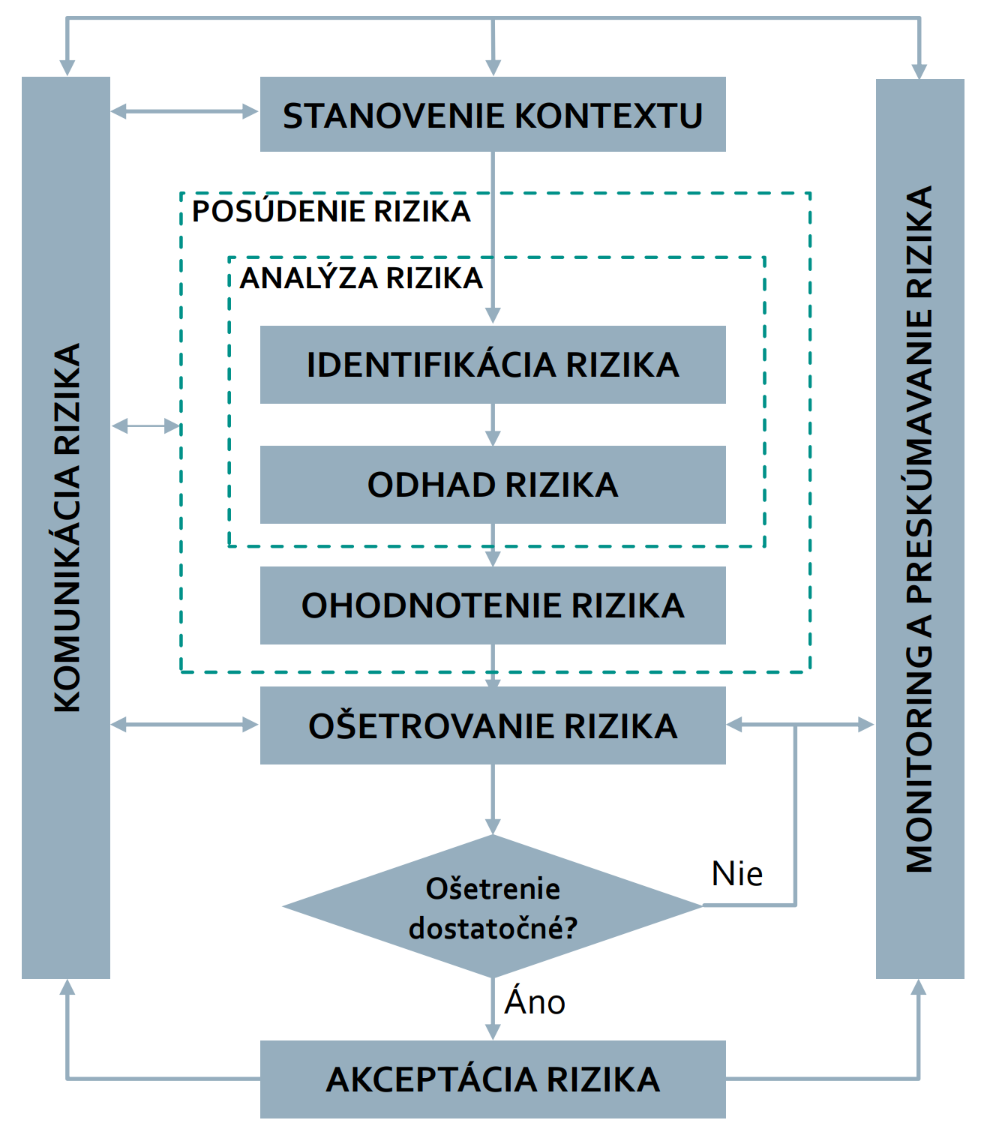
\includegraphics[width=0.5\linewidth]{iso27k5risk.png}
        \caption{Všeobecná schéma procesu riadenia rizík informačnej bezpečnosti podľa ISO/IEC 27005}
        \label{fig:placeholder}
    \end{figure}
    \subsection{Vzdelávanie, tréning a zvyšovanie povedomia v informačnej bezpečnosti}
    \subsection{Riešenie bezpečnostných incidentov. Kontinuita činnosti. Certifikácia ISMS}

    \subsection*{Prehľad legislatívy}
    \begin{sidewaystable}
    \centering
    \scriptsize
    \renewcommand{\arraystretch}{1.5}
    \begin{tabular}{|p{5cm}|p{8cm}|p{7cm}|}
    \hline
    \rowcolor[HTML]{C0C0C0}
    \textbf{Názov / Norma} & \textbf{Čo pokrýva (Rozsah)} & \textbf{Súvislosti / Nadväznosti / Transpozície} \\ \hline
    
    ISO/IEC 27001:2022 & Medzinárodná norma pre budovanie a správu ISMS. Zahŕňa riadenie rizík, opatrenia z prílohy A, neustále zlepšovanie (cyklus PDCA). & Základ pre mnohé národné normy (napr. STN ISO 27001). Plne kompatibilná s BSI IT-Grundschutz. Nepriamo podporuje súlad s GDPR a NIS2. \\ \hline
    
    BSI IT-Grundschutz (normy 200-1 až 200-4) & Modulárny a metodický rámec od BSI (Nemecko) na implementáciu ISMS.  \begin{itemize}
        \item 200-1: Zásady ISMS
        \item 200-2: Prístupy (základná, štandardná, jadrová ochrana)
        \item 200-3: Analýza rizík
        \item 200-4: Riadenie kontinuity činností (BCM).
    \end{itemize} & Vzťahuje sa na ISO/IEC 27001. Uznávaný v celej EÚ. Podporuje súlad s GDPR, NIS2 a CER. Často používaný vo verejnom sektore a kritickej infraštruktúre. \\ \hline
    
    STN EN ISO/IEC 27001, 27002, 27005, 27017, 27018, 22301 & Slovenské verzie ISO noriem pre bezpečnosť, cloud, riziká, súkromie a kontinuitu. & Ekvivalent medzinárodných ISO noriem. Slúži ako základ pre regulované sektory a certifikáciu. \\ \hline
    
    Zákon č. 69/2018 Z.z. (Zákon o kybernetickej bezpečnosti) & efinuje riešenie kybernetickej (a infor-
mačnej) bezpečnosti v SR  & Transpozícia NIS1, novelizovaný v roku 2024 (NIS2). Súvisí s GDPR, zákonom o verejnej správe a ISMS rámcami. \\ \hline


% Upravuje povinnosti v oblasti kybernetickej bezpečnosti pre prevádzkovateľov základných služieb vrátane riadenia rizík, hlásenia incidentov a reakcie na ne. Určuje úlohy orgánov verejnej moci, tímov CSIRT a audity. Vzťahuje sa aj na zahraničných poskytovateľov digitálnych služieb, ak pôsobia na Slovensku alebo cielia na slovenských používateľov bez určeného zástupcu. Nevzťahuje sa na utajované systémy, spravodajské služby, trestné konania a infraštruktúru finančného sektora.
    
    Novela 2024/2025 (implementácia NIS2) & Transpozícia smernice NIS2 (2022/2555). Rozširuje pôsobnosť, zvyšuje zodpovednosť manažmentu, zavádza prísnejšie sankcie a požiadavky na riadenie rizík. & Silná väzba na ISO/IEC 27001 a BSI IT-Grundschutz. Vyžaduje formálne ISMS, BCM a hlásenie incidentov. \\ \hline
    
    Zákon č. 367/2024 Z.z. – zákon o odolnosti kritických subjektov & Transpozícia smernice CER (2022/2557). Zameriava sa na infraštruktúrnu odolnosť sektorov (energia, doprava, zdravotníctvo). & Dopĺňa NIS2. Prekryv v sektoroch. BCM (BSI 200-4) a ISMS podporujú splnenie požiadaviek. \\ \hline
    
    Zákon č. 18/2018 Z.z. – Ochrana osobných údajov (GDPR) & Transpozícia GDPR do slovenského práva. Upravuje spracovanie osobných údajov, zodpovednosť, DPIA, incidenty. & Podporovaný ISO/IEC 27701 (rozšírenie k ISO 27001). BSI IT-Grundschutz pokrýva súvisiace opatrenia. \\ \hline
    
    Zákon č. 95/2019 Z.z. – IT systémy vo verejnej správe & Upravuje životný cyklus, bezpečnosť a interoperabilitu IT systémov verejnej správy. & Vyžaduje súlad s kybernetickou a dátovou legislatívou. Podporuje ISMS princípy (ISO, BSI). \\ \hline
    
    Katalóg opatrení IT-Grundschutz (Bausteine) & Modulárny katalóg technických a organizačných opatrení pre IS, siete, aplikácie a personál. & Súčasť BSI štandardov. Mapovaný na prílohu A z ISO/IEC 27001. Podporuje súlad s GDPR, NIS2 a CER. Verejne dostupný (bsi.bund.de). \\ \hline
    
    \end{tabular}
    \caption{Prehľad štandardov ISMS, BSI IT-Grundschutz a legislatívy SR/EÚ}
    \label{tab:isms-legislativa}
    \end{sidewaystable}

    \begin{figure}[htbp]
\centering
\begin{tikzpicture}[
  node distance=1.9cm and 2cm,
  box/.style={draw, rectangle, rounded corners, text width=4.2cm, align=center, font=\footnotesize, fill=blue!10},
  law/.style={draw, rectangle, rounded corners, text width=4.7cm, align=center, font=\footnotesize, fill=red!10},
  directive/.style={draw, rectangle, text width=3.8cm, align=center, font=\footnotesize, fill=green!10},
  arrow/.style={thick, ->, >=Stealth}
]

% Directives (Left Column)




% Laws (Right Column)
\node[directive] (nis2) at (0,0) {NIS2 (2022/2555)};
\node[law, below=of nis2] (zakon69) {Zákon č. 69/2018 Z.z.\\+ novela 2024 (Kybernetická bezpečnosť)};
\node[law, below=of zakon69] (zakon95) {Zákon č. 95/2019 Z.z.\\(IT vo verejnej správe)};
\node[directive, below=of zakon95] (gdpr) {GDPR (2016/679)};
\node[law, below=of gdpr] (zakon18) {Zákon č. 18/2018 Z.z.\\(GDPR)};
\node[directive, below=of zakon18] (cer) {CER (2022/2557)};
\node[law, below=of cer] (zakon367) {Zákon č. 367/2024 Z.z.\\(Odolnosť kritických subjektov)};

% Standards (Bottom row, center)
\node[box, right=of zakon69] (iso27001) {ISO/IEC 27001:2022};
\node[box, below=3cm of iso27001] (grundschutz) {BSI IT-Grundschutz\\(200-1 až 200-4)};
\node[box, below=3cm of grundschutz] (iso27002) {ISO 27002, 27005,\\27701, 22301};

% Transposition arrows
\draw[arrow] (nis2) -- node[midway, sloped, above, font=\scriptsize] {Transpozícia} (zakon69);
\draw[arrow] (cer) -- node[midway, sloped, above, font=\scriptsize] {Transpozícia} (zakon367);
\draw[arrow] (gdpr) -- node[midway, sloped, above, font=\scriptsize] {Transpozícia} (zakon18);

% Compliance support from standards
\draw[arrow, bend right=20] (iso27001) to node[midway, sloped, above, font=\scriptsize] {Podpora súladu} (zakon69);
\draw[arrow, bend left=10] (grundschutz) to node[midway, sloped, below, font=\scriptsize] {Podpora súladu} (zakon69);
\draw[arrow, bend left=100] (grundschutz) to node[midway, sloped, above, font=\scriptsize] {Opatrenia pre odolnosť} (zakon367);
\draw[arrow, bend left=10] (iso27002) to node[midway, sloped, below, font=\scriptsize] {Opatrenia pre odolnosť} (zakon367);

\draw[arrow, bend left=15] (grundschutz) to node[midway, sloped, above, font=\scriptsize] {Opatrenia pre GDPR} (zakon18);
\draw[arrow, bend left=15] (iso27002) to node[midway, sloped, below, font=\scriptsize] {Opatrenia pre GDPR} (zakon18);

\draw[arrow, bend left=15] (grundschutz) to node[midway, sloped, below, font=\scriptsize] {Podpora IS/IT} (zakon95);

% Relationships among standards
\draw[arrow] (iso27001) -- node[midway, sloped, above, font=\scriptsize] {Kompatibilita} (grundschutz);
\draw[arrow] (grundschutz) -- node[midway, sloped, above, font=\scriptsize] {Rozšírenie / moduly} (iso27002);

\end{tikzpicture}
\caption{Vzťahy medzi normami ISMS, legislatívou SR a smernicami EÚ.}
\label{fig:isms-map}
\end{figure}
}

\examquestion{Bezpečný vývoj aplikácií}{
    \subsection{Zraniteľnosti lokálnych a webových aplikácií, opatrenia}
    \subsection{Bezpečné programovanie – princípy, príklady vo vybraných programovacích jazykoch}
    \subsection{Revízia kódu, statická analýza kódu}
}

\end{document}
